\setchapterpreamble[u]{\margintoc}
\chapter*{Introducción}
\labch{introduction_spanish}
\label{sec:introduction_spanish}

\lettrine[findent=0pt, lines=3]{\fbox{\textbf{L}}}{ } a observación de procesos en el mundo real ayuda a controlar, predecir y optimizar las actividades que dependen de ellos y, por tanto, a actuar en función de los datos analizados. Existen numerosos sensores que posibilitan esta tarea, los cuales pueden clasificarse, al menos, en función de la distancia de detección, la gama de longitudes de onda captadas por los detectores del dispositivo y el mecanismo de adquisición de datos, ya sea pasivo o activo. Las dos últimas clasificaciones se basan en el funcionamiento del dispositivo. Sin embargo, la primera categoría de clasificación de los objetivos y el área de aplicación que persigan tanto los investigador como el consumidor final. Igualmente, también influyen el presupuesto del que disponemos, y el tamaño y las condiciones ambientales de la zona de estudio, entre otros factores. A pesar de que es posible utilizar sensores que precisan del contacto con la superficie objectivo para medir variables como humedad, temperatura o cantidad de lluvia, estos requieren un alto grado de mantenimiento y son más propensos a deteriorarse en condiciones ambientales adversas \cite{silva_low-cost_2019, morais_versatile_2021}. Además, en lugar de cubrir grandes áreas, cada uno de estos sensores comunica dentro y fuera de una red de sensores medidas procedentes de posiciones muy específicas. En un espacio continuo e infinito, se discretiza su monitorización mediante un número variable de posiciones. La disposición de estos sensores, tanto lógica como física, debe ser cuidadosamente diseñada para permitir la intra y extra-comunicación, involucrando nodos en diferentes niveles de la topología propuesta. Por lo tanto, estas tecnologías no son apropiadas para implementar sistemas de monitorización constante y en tiempo real cubriendo todo un área. 

\marginnote[.1cm]{Las técnicas de \textbf{teledetección} evitan las limitaciones espaciales que encontramos en otros dispositivos que aportan medidas mediante un contacto directo con la superficie objetivo o la atmósfera. } 
Las técnicas de teledetección ayudan a mitigar algunas de las desventajas mencionadas adquiriendo datos desde plataformas aéreas, satelitales e incluso terrestres; en cualquier caso, no requieren de un contacto directo, sino que simplemente observan y capturan información. La teledetección se define como el arte y la ciencia de adquirir información de objetos y fenómenos sin estar en contacto directo con éstos \cite{lillesand_remote_2015}. De manera similar al ojo humano, los datos se adquieren mediante impulsos generados por estímulos de la luz, los cuales corresponden a unas longitudes de onda específicas. Al menos dos componentes se ven involucradas en el proceso de lectura: sensores y aquellas plataformas en las que éstos se acoplan. Los primeros serán objetivo de discusión a lo largo de todo este trabajo, mientras que las plataformas son muy variadas, aunque en un comienzo hacian mención principalmente a satélites. El término \textbf{teledetección} se origina en la década de 1960, acuñado por Eveleyn Pruitt, para referirse a instrumentos satelitales y aéreos que posibilitan medir la radiancia reflejada y emitida. No obstante, las técnicas topográficas fueron sugeridas inicialmente en 1849, y llevadas a la práctica en 1858 por F. Tournachon en un globo aerostático, sobrevolando Francia. Desde estos comienzos, el tamaño de las cámaras se ha reducido, haciéndolas más cómodas de utilizar. Influenciados por ciertos acontecimientos históricos y el conocimiento hasta ese momento recabado, otros medios aéreos empleados para estas tareas fueron cometas (1906; Figura \ref{fig:san_francisco_kite_spanish}), aves (1909), y por último, aeronaves (1908). 

\begin{figure}[!ht]
	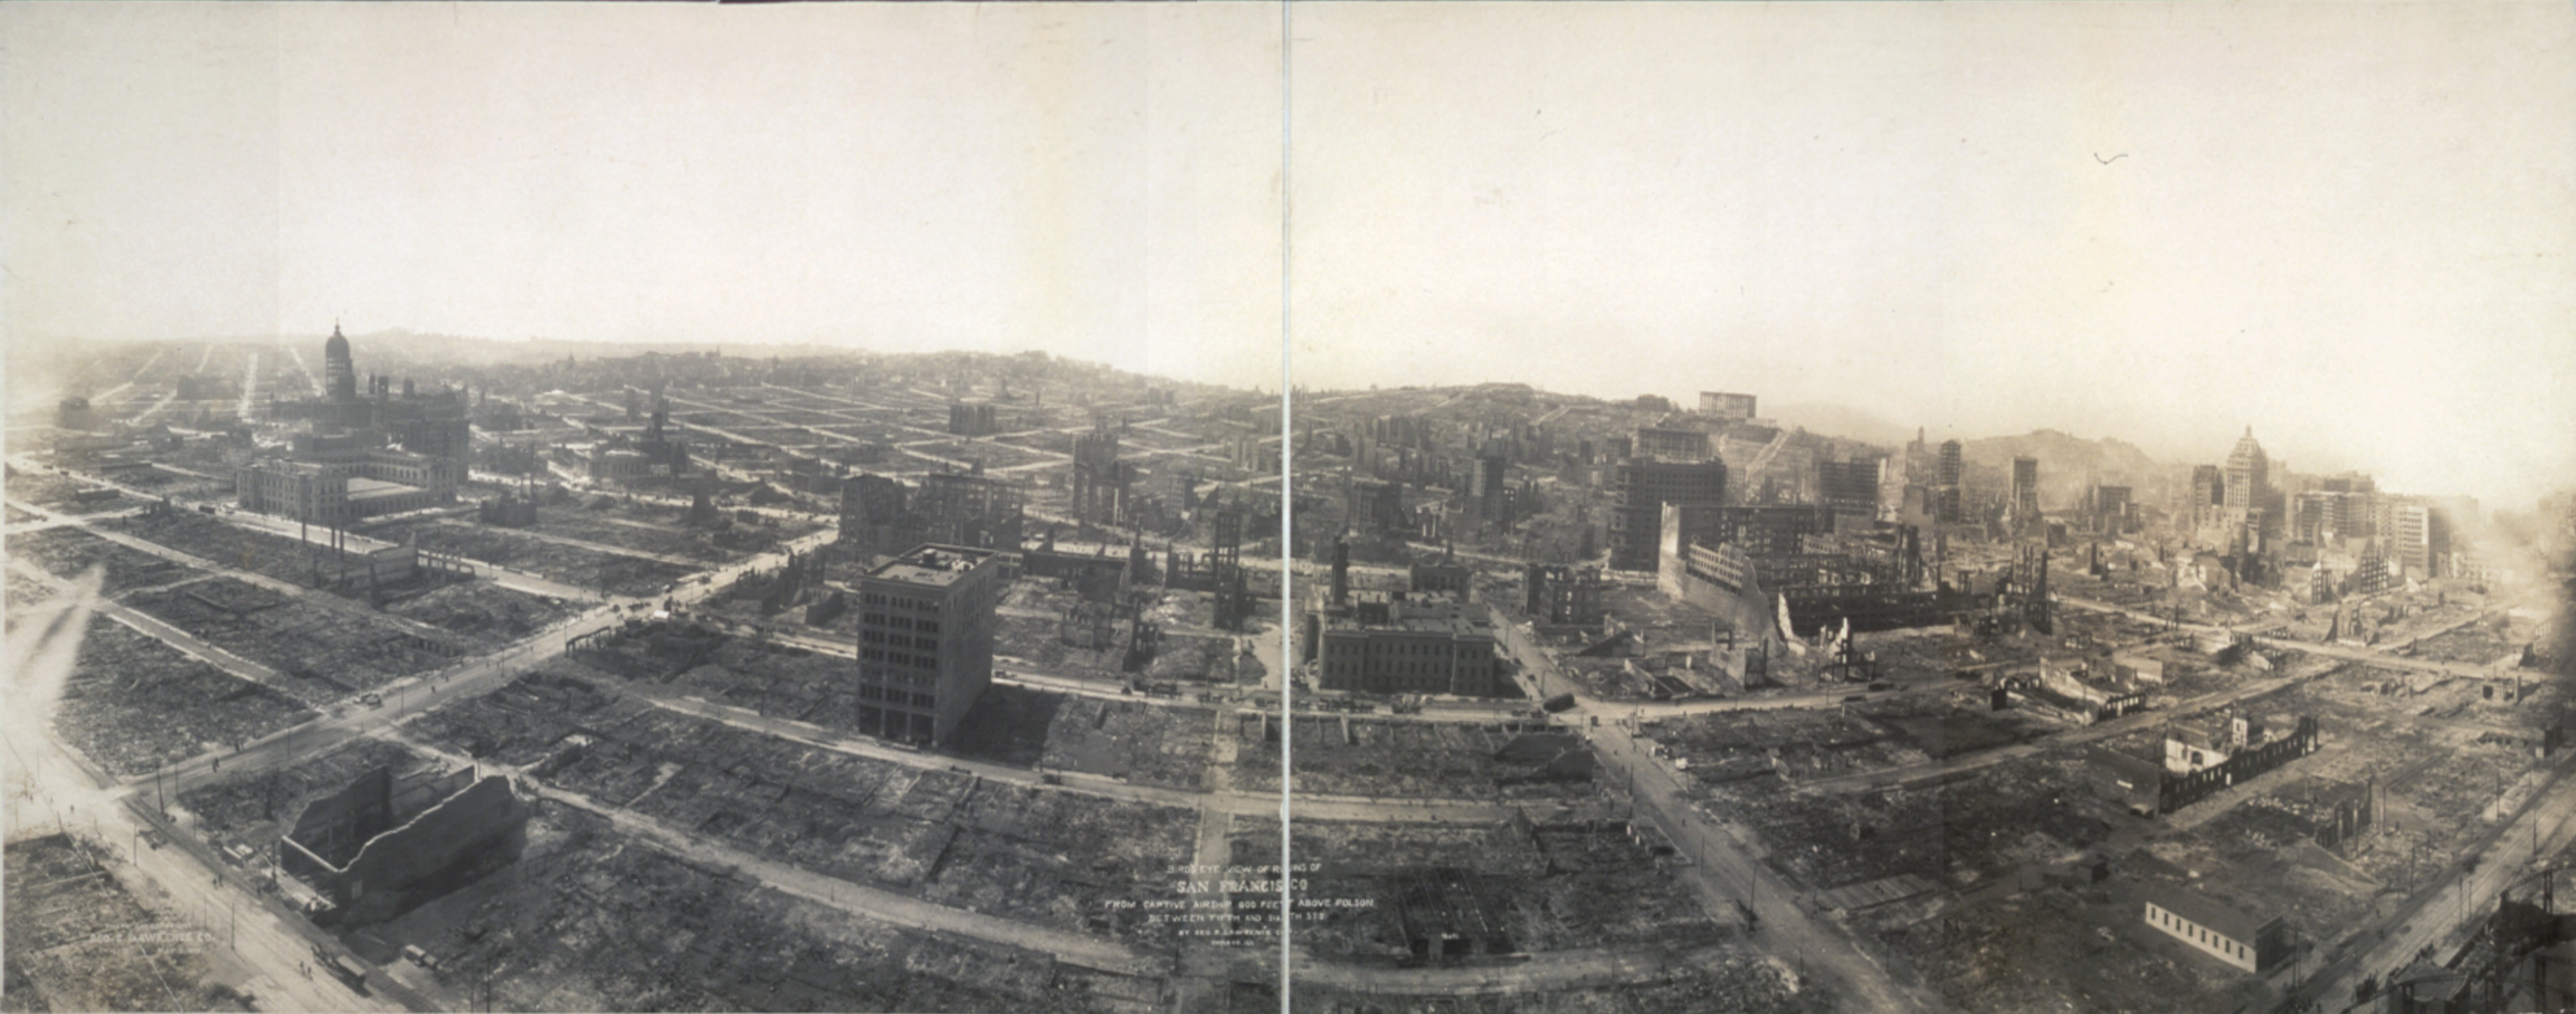
\includegraphics{figs/introduction/san_francisco_kitecamera.jpg}
	\caption{Fotografía de San Francisco después del terremoto de 1906, capturada desde una camera soportada por siete cometas. }
    \label{fig:san_francisco_kite_spanish}
\end{figure}

La imagen por satélite, tal y como se conoce hoy en día, es posible gracias a la idea inicial de Konstantin Tsiolkovsky de utilizar cohetes para explorar el espacio, publicada bajo el título \textit{Exploring Space using jet propulsion devices}. Esta idea desembocó en el primer lanzamiento con éxito, el satélite Sputnik en 1957, e igualmente contribuyó al desarrollo de satélites para la vigilancia atmosférica. El satélite de observación por televisión e infrarrojos (TIROS) entró en funcionamiento en 1960, integrando un pequeño sistema de infrarrojos y una cámara con un ángulo de visión muy reducido para captar datos en las longitudes de onda visibles. En 1978, TIROS-N (nuevo) supuso un cambio radical en los satélites y sus sensores acoplados. Esta nave espacial integraba un radiómetro de alta resolución (1 \si{\kilo\\metro}) y otros cuatro canales (visible, infrarrojo cercano, infrarrojo medio e infrarrojo térmico). En la actualidad, una versión avanzada de estos satélites sigue operativa bajo el nombre de AVHRR-3 (Advanced Very High-Resolution Radiometer) con una resolución similar, aunque captura seis bandas espectrales diferentes, en lugar de sólo cuatro \cite{national_oceanic_and_atmospheric_administration_avhrr3_nodate}.   

\marginnote[.1cm]{Un amplio repositorio de misiones satelitales recientes se encuentra en el Earth Observation Portal, mantenido por la Agencia Espacial Europea \cite{earth_observation_portal_earth_nodate}.} 
\begin{marginfigure}[3.0cm]
	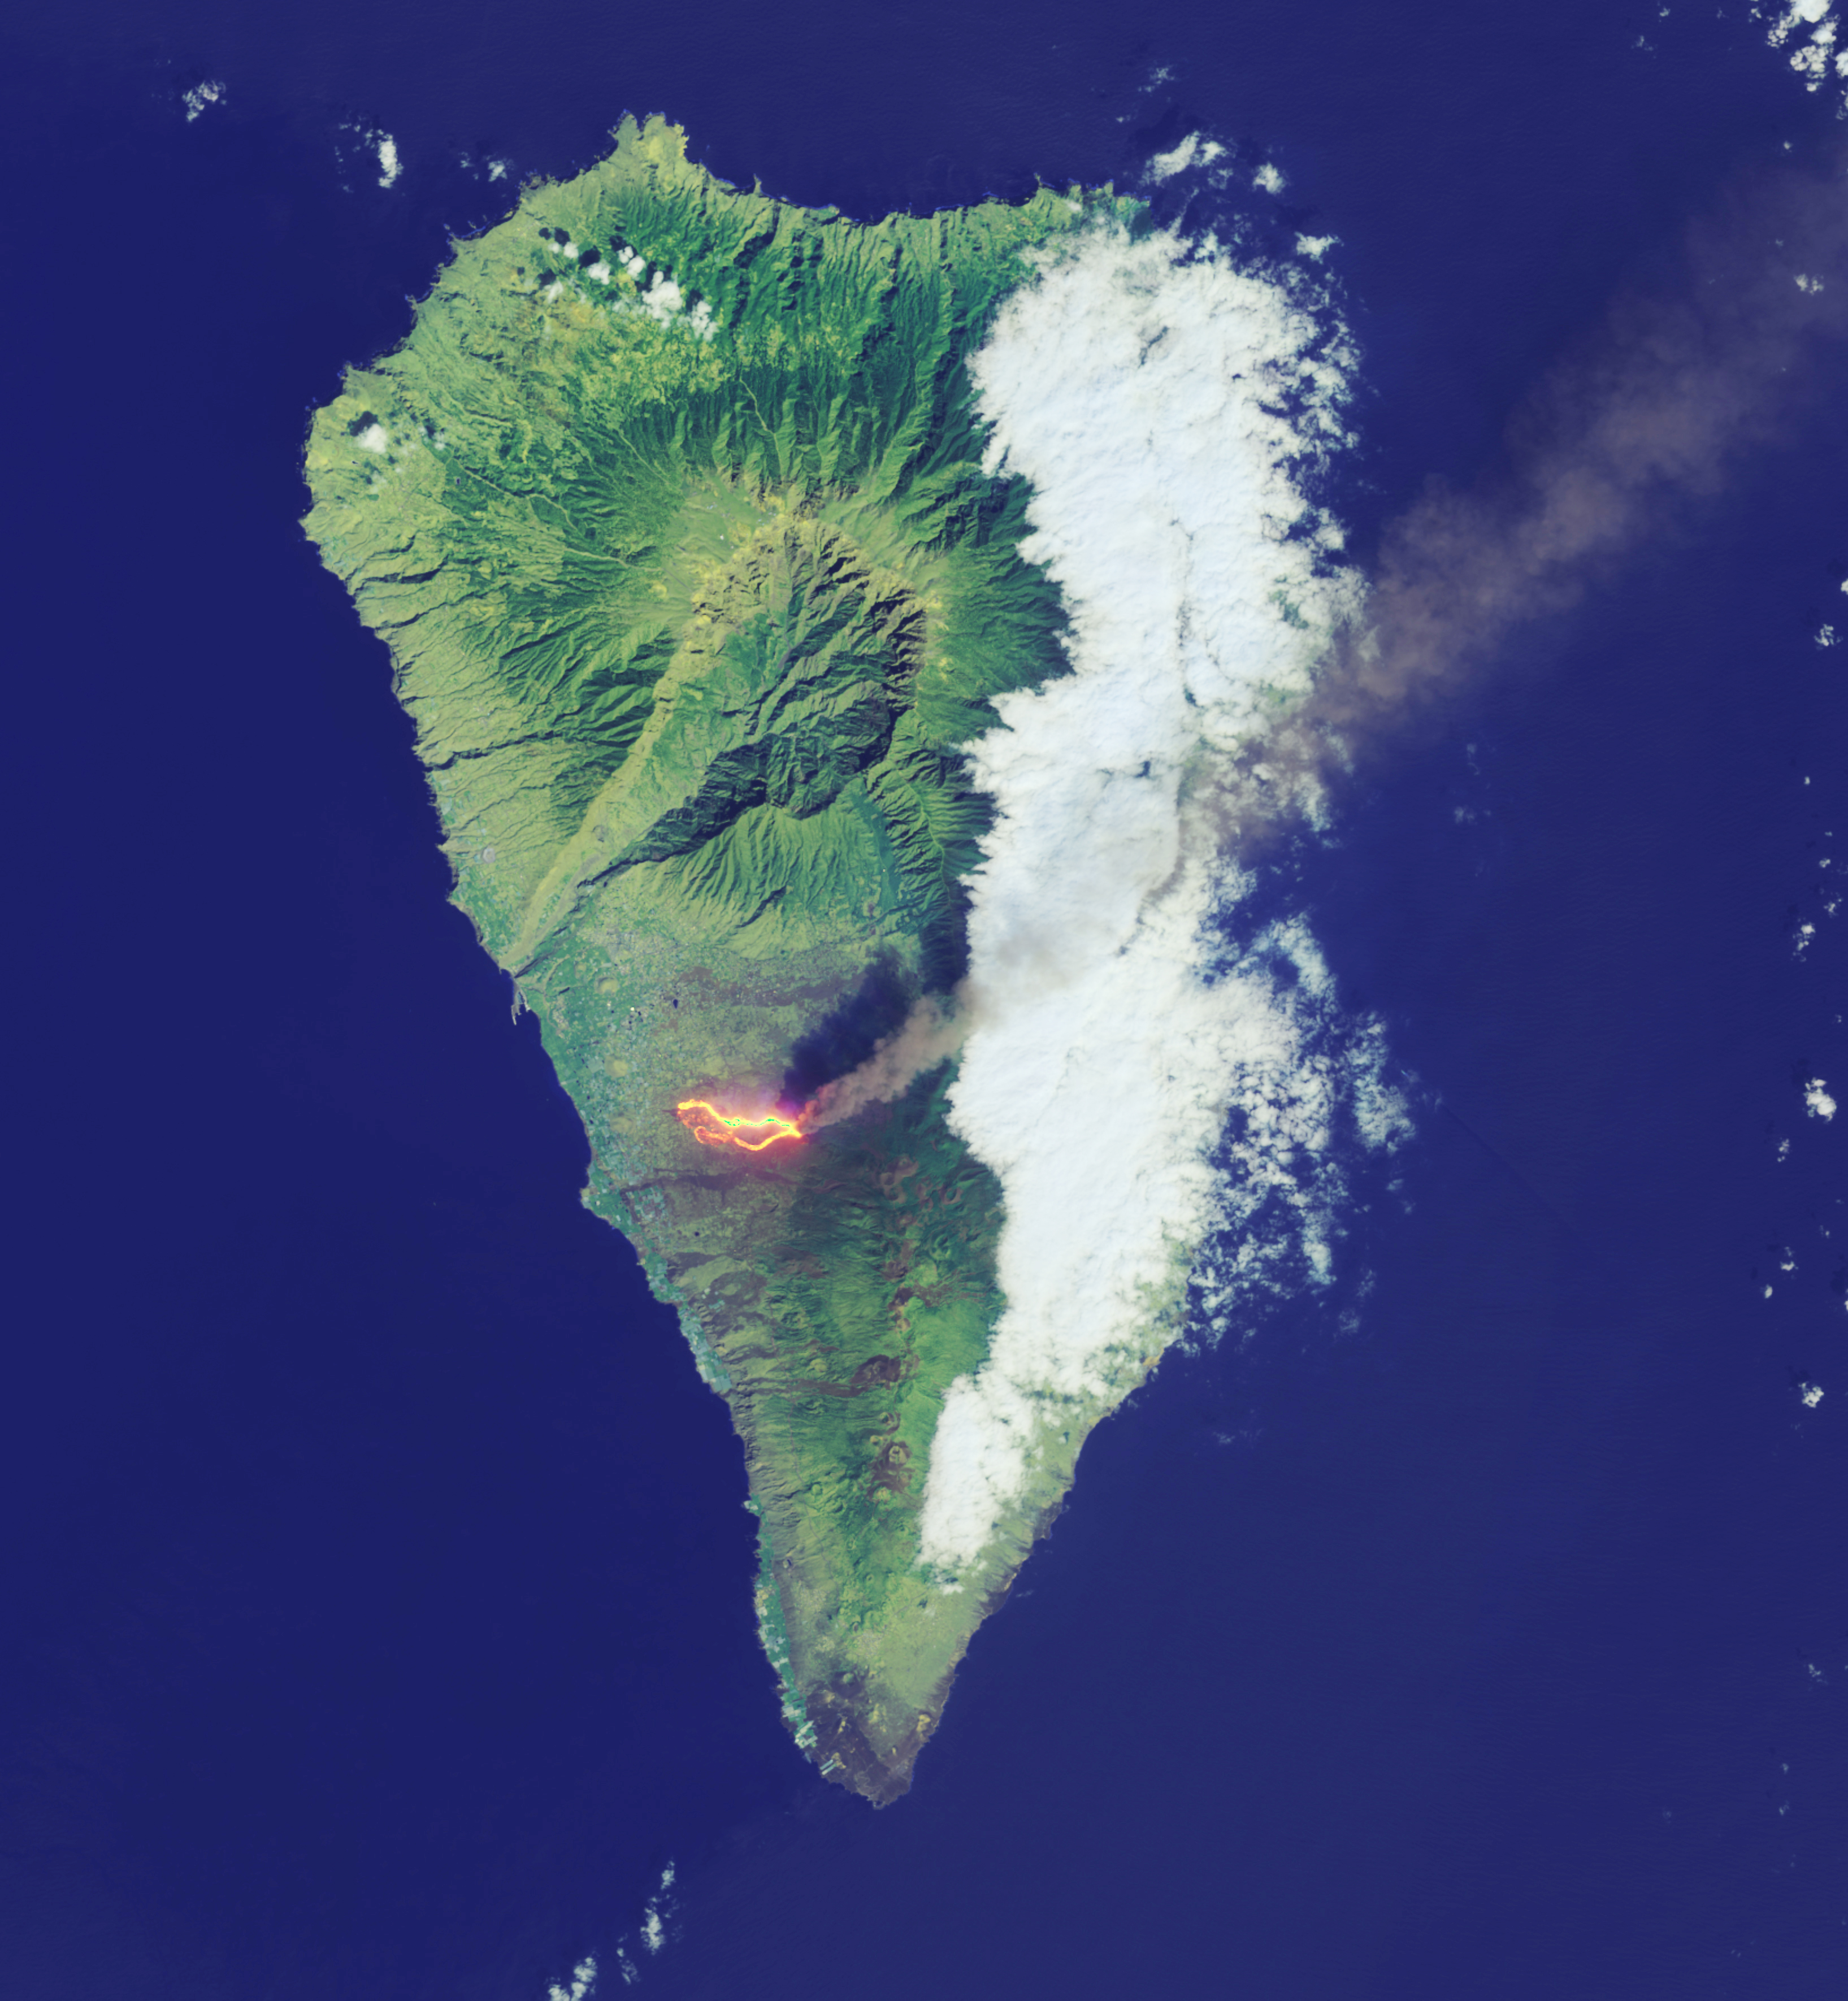
\includegraphics{figs/introduction/landsat8_lapalma.jpg}
	\caption{Erupción del volcán Cumbre Vieja observada desde la misión Landsat-8 \cite{nasa_earth_observatory_lava_2021}.}
	\label{fig:la_palma_landsat8_spanish}
\end{marginfigure}
Entre los proyectos de satélite actualmente operativos, Landsat es el que proporciona la mayor colección de datos de teledetección adquiridos de forma continua. Se utilizó por primera vez como parte del programa NIMBUS de la NASA y en la actualidad hay dos satélites activos, Landsat 8 y Landsat 9, mientras que los otros siete han sido dados de baja o está previsto su desmantelamiento en los próximos años (Landsat 7). La carga útil de Landsat 9 consta de dos sensores: Operational Land Imager (OLI-2) y un sensor infrarrojo térmico (TIRS-2). Cada día se recogen un total de 740 escenas con 11 bandas, incluyendo roja, azul, verde, infrarroja cercana, infrarroja de onda corta, térmica, pancromática, costera y de cirros, con una resolución de 15 \si{\meter} a 100 \si{\meter}. Otros programas de satélites destacados son el Satélite de Recursos Terrestres China-Brasil (CBERS) y el programa Copernicus, financiado por la Comisión Europea. El satélite CBERS-04A está equipado con tres sensores que capturan cinco intervalos espectrales diferentes con una resolución espacial entre 2 \si{\meter} y 55 \si{\meter}. \cite{instituto_nacional_de_pesquisas_espaciais_inpecbers_2019}. Por su parte, la misión Sentinel-2 obtiene 13 bandas en el espectro visible, onda corta e infrarrojo cercano (ver Figura \ref{fig:sentinel2_spanish}) con una resolución espacial que oscila entre los 10 \si{\meter} y los 60 \si{\meter} \cite{european_environment_agency_eu_2017}. Su periodo de tiempo para revisitar el mismo punto de la Tierra es de diez días, en comparación con los 16 días que necesita Landsat 9 o los 31 días de CBERS-04A.

\begin{figure}[!ht]
	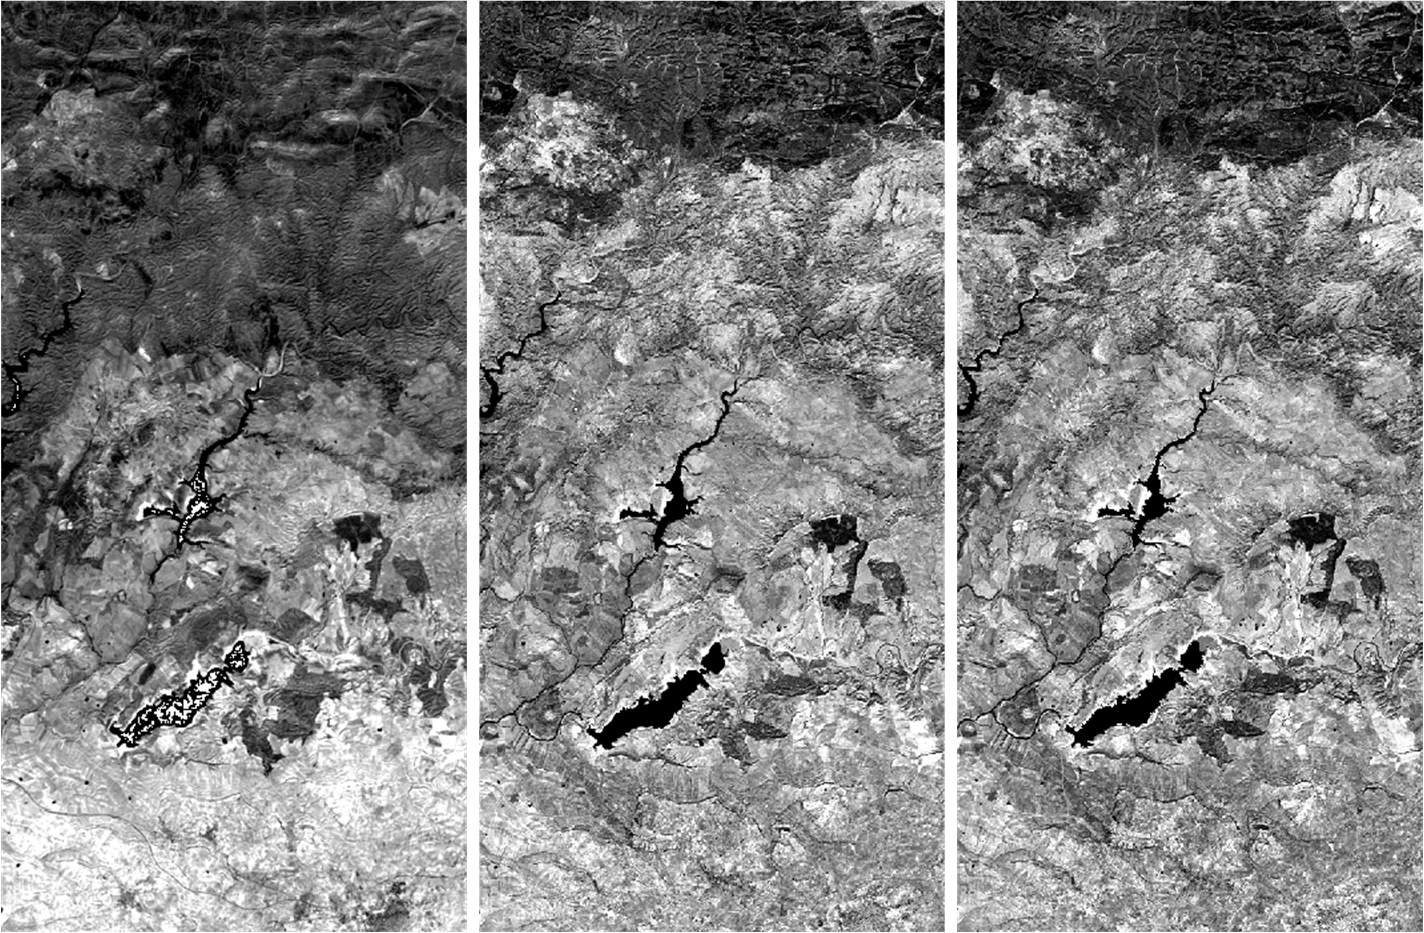
\includegraphics{figs/introduction/sentinel2_bands.png}
	\caption{Tres bandas en el infrarrojo cercano capturadas por la misión Sentinel-2 (banda 9, 935-955 \si{\micro\meter}, banda 11, 1567-1658 \si{\micro\meter}, y banda 12, 2114-2889 \si{\micro\meter}). }
    \label{fig:sentinel2_spanish}
\end{figure}

Por tanto, las imágenes por satélite son más adecuadas para monitorizar cambios a larga escala, utilizando series temporales que abarcan meses, años e incluso décadas. Estos datos permiten comprender la interacción entre el hombre y la naturaleza, así como el impacto de los fenómenos naturales (Figura \ref{fig:la_palma_landsat8_spanish}). Algunas aplicaciones de los conjuntos de datos obtenidos por misiones de satélite son el control de: uso del suelo, deforestación, cambios en la superficie terrestre y asentamientos urbanos \cite{asokan_change_2019}. No obstante, la resolución espacial y el período de revisita de los programas de satélites no comerciales dificultan su aplicabilidad a tareas de seguimiento que requieran de un alto nivel de detalle (LOD). Este nivel de detalle puede referirse a la resolución espacial, a la resolución temporal o a ambas, que son las principales limitaciones de las imágenes por satélite, además de su coste. A pesar de estas desventajas, el uso de imágenes por satélite está en aumento debido a la disminución constante de la distancia de muestreo terrestre (GSD) y a los bajos periodos de revisita de los mismos puntos (véase la figura \ref{fig:scopus_search_platforms_spanish}). Por ejemplo, el satélite comercial Pléiades Neo (VHR-2020) de Airbus Defense \& Space \cite{airbus_pleiades_2021} es capaz de adquirir diariamente siete bandas con una GSD de 30 \si{\centi\meter}. Incluso para las misiones gubernamentales, el ciclo de repetición suele ser reducido, ya que varias misiones gemelas podrían estar activas en el mismo momento con instrumentos y órbitas similares. Así, el desfase en las trayectorias de Landsat-8 y Landsat-9 permite adquirir datos del mismo punto cada 8 días \cite{masek_landsat_2020}. Aun así, obtener datos de misiones espaciales puede llegar a ser mucho más prohibitivo que el resto de técnicas en términos económicos.

\begin{figure}[!ht]
	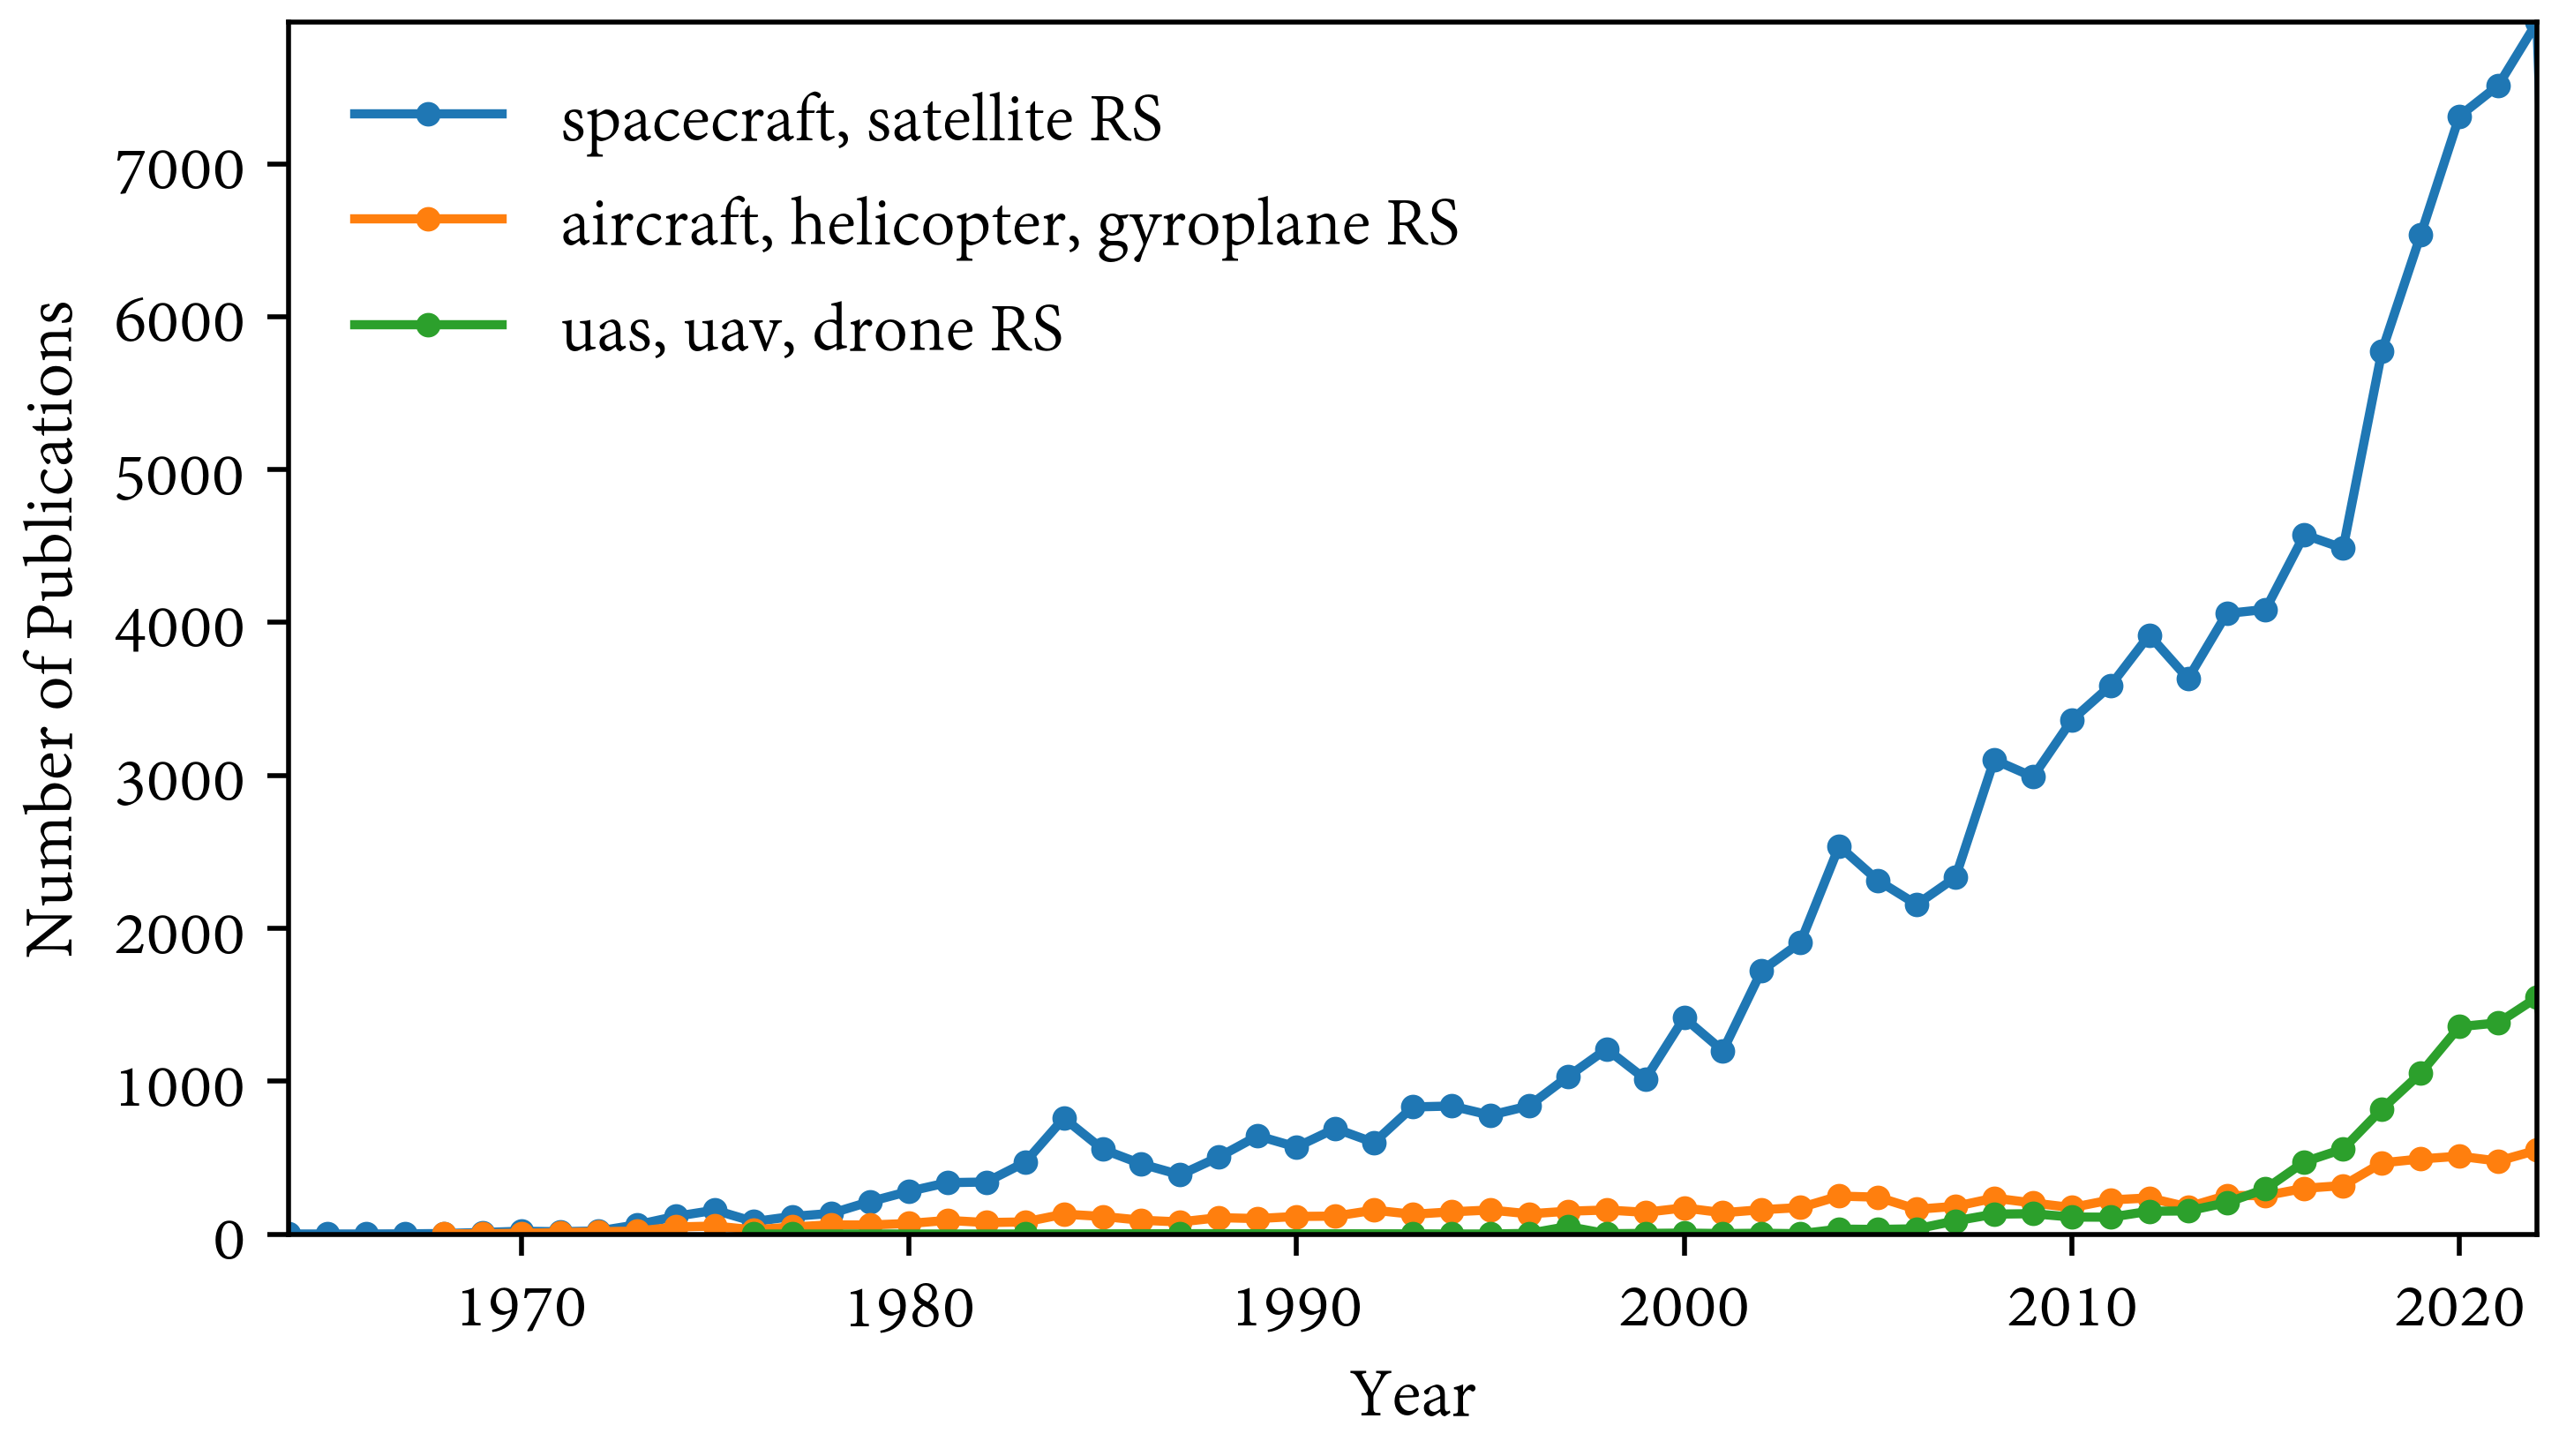
\includegraphics[width=\linewidth]{figs/introduction/platform_timeline.png}
	\caption{Número de artículos relacionados con diferentes plataformas de teledetección. Las búsquedas de Scopus fueran las siguientes: $(p_1 \lor p_2 ... \lor p_n) \land (\textit{remote} \hspace{1mm} \land \hspace{1mm} \textit{sensing})$, donde $p_i$ es una de las plataformas en la leyenda. }
    \label{fig:scopus_search_platforms_spanish}
\end{figure}

\begin{marginfigure}[.7cm]
	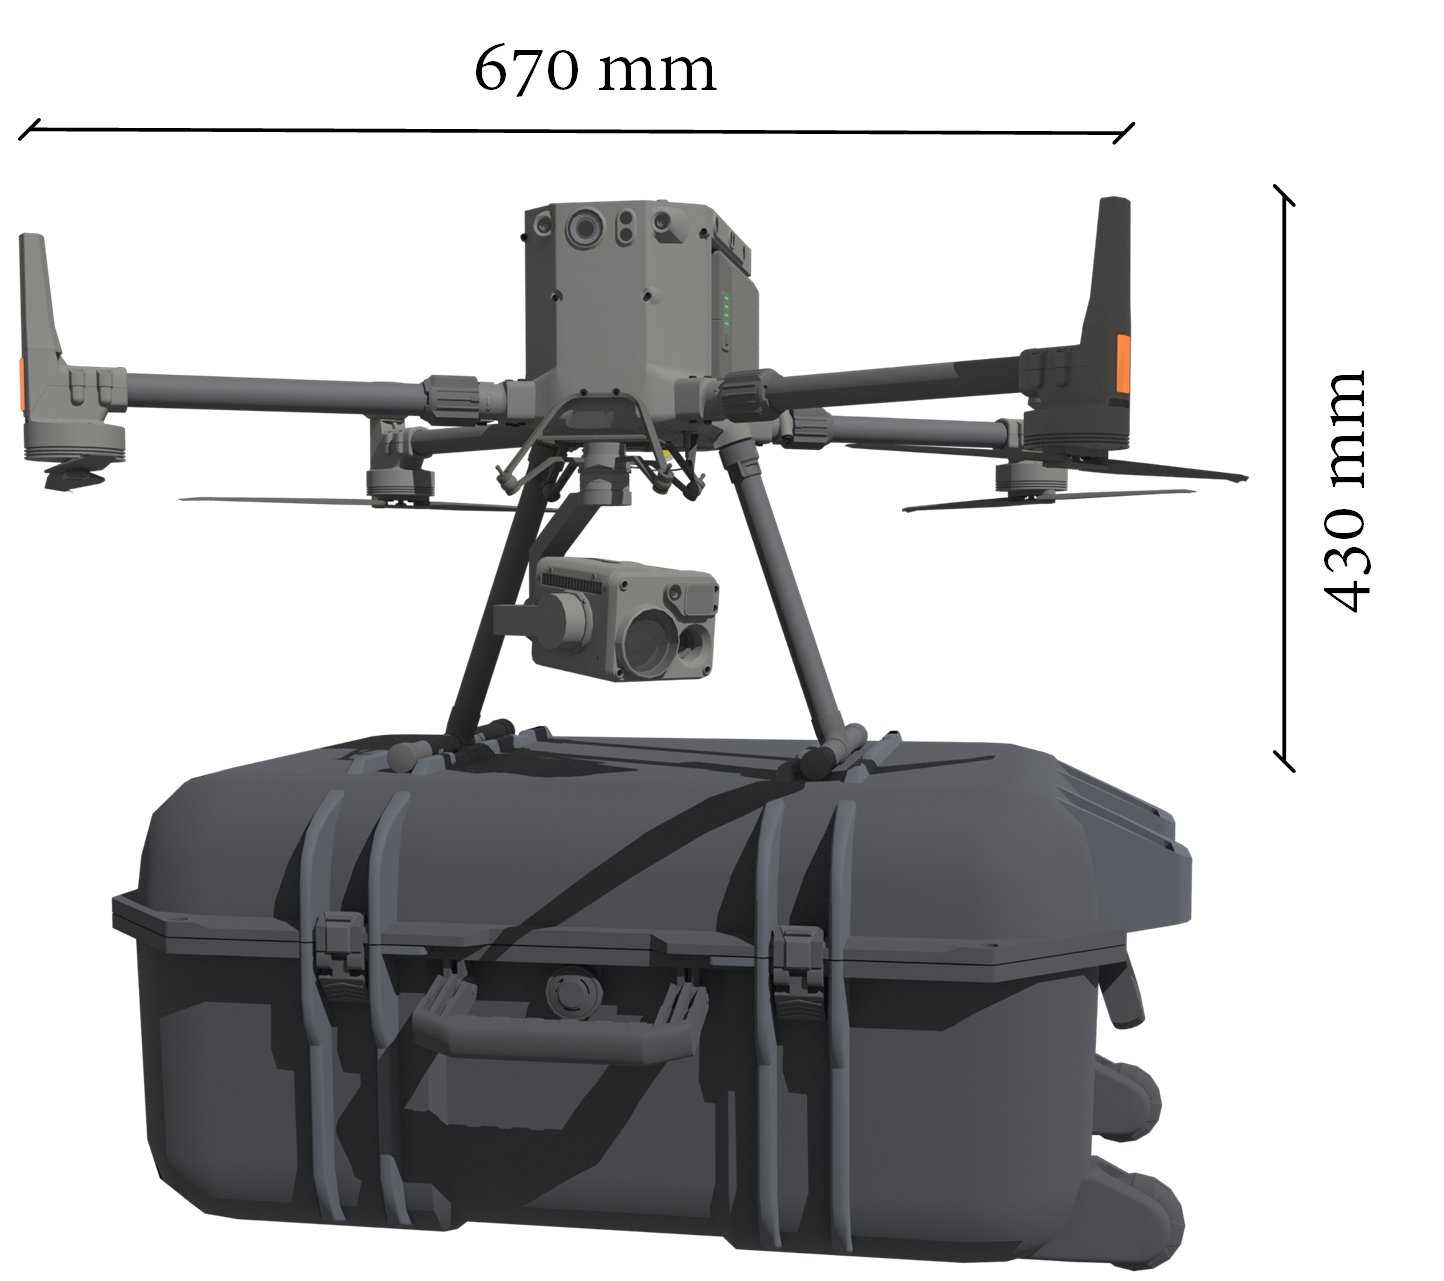
\includegraphics{figs/introduction/dji300.png}
	\caption{Quadcóptero Matrice 300 RTK, acoplado con un dispositivo dual RGB-termográfico. }
	\label{fig:dji300_spanish}
\end{marginfigure}
Además de las dificultades técnicas, la resolución de las misiones de satélite estaba restringida hasta hace bien poco por algunos gobiernos. Estas restricciones, así como las limitaciones descritas, condujeron al uso de plataformas alternativas. Además de satélites, las aeronaves (ala fija y helicópteros), los sistemas aéreos no tripulados (UAS) (figura \ref{fig:dji300_spanish}) y otras plataformas terrestres (móviles y estáticas con detección próxima) son las más frecuentes \cite{lillesand_remote_2015}. La elección de cualquiera de ellas siempre implica balanear maniobrabilidad, cobertura terrestre, resolución espacial, precisión espacial, coste y campo de visión (FOV). Sin embargo, los drones han ido ganando interés en la última década al pasar de ser simples herramientas militares a principios de la década de 2000, a sistemas fáciles de desplegar, pequeños y de bajo coste, ampliando así su aplicabilidad a operaciones civiles o investigación. Estas plataformas abarcan desde aeronaves del tamaño de una mano hasta otras de gran tamaño que pueden ser controladas por operadores humanos o ser parcial o incluso totalmente autónomas. La figura \ref{fig:dji300_spanish} muestra un dron estándar diseñado por DJI que puede transportar hasta 2,7\si{\kilo\gram}, con unas dimensiones de $501 \times 403 \times 252$ \si{\milli\meter}.

\begin{figure}[!ht]
	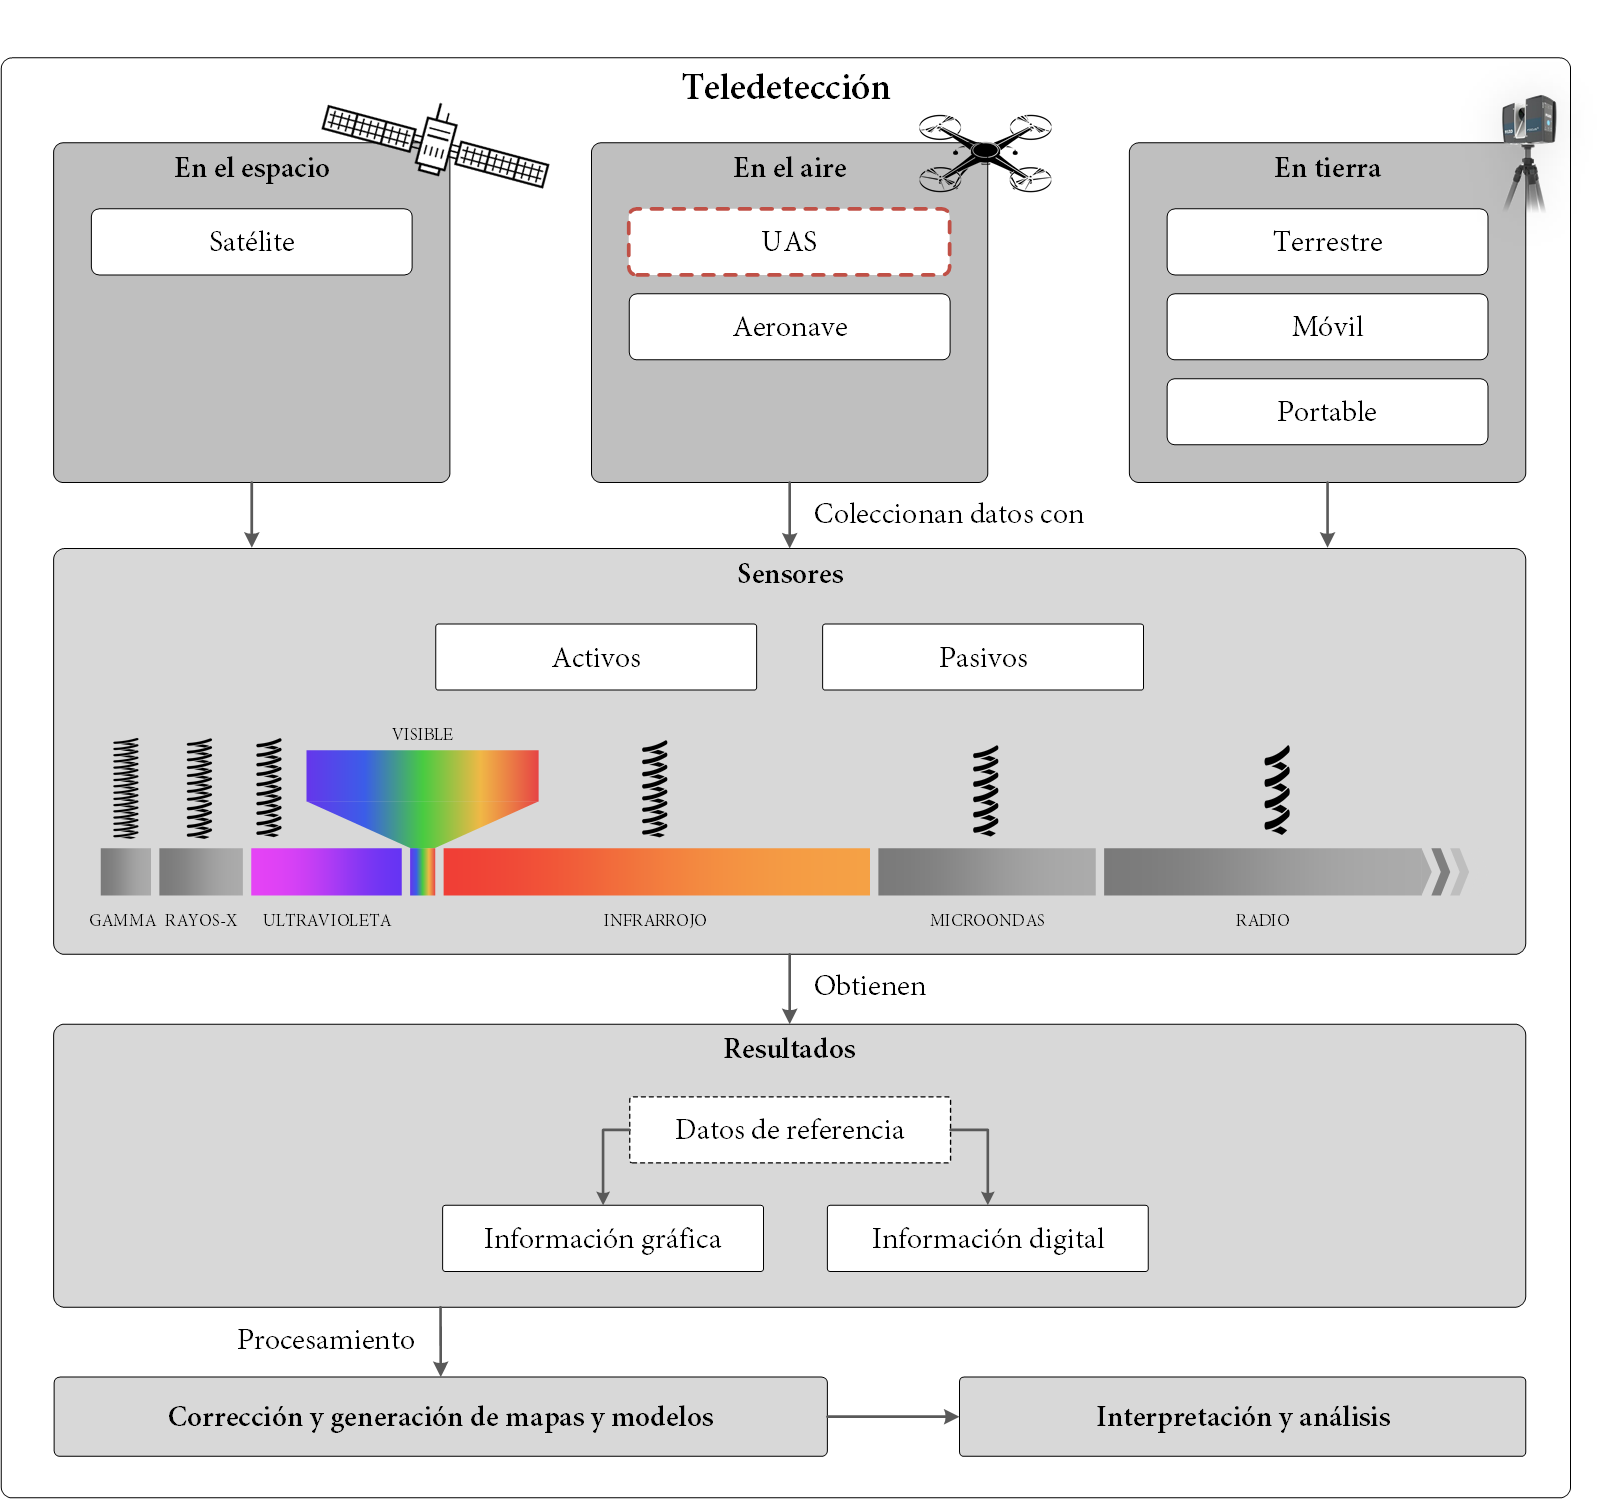
\includegraphics{figs/introduction/introduction_scheme_spanish.png}
	\caption{Procedimiento general de adquisición de datos con plataformas y sensores de teledetección. En primer lugar, los sensores se acoplan en vehículos espaciales, aéreos y terrestres o son manejados por humanos, ya sea llevándolos como mochila o en la mano. A continuación, los productos de los sensores pueden agruparse en resultados gráficos y numéricos, aunque la mayoría de ellos producen ambos tipos de datos. Por último, los productos de los sensores se procesan e interpretan para proporcionar a los usuarios valiosos análisis. }
    \label{fig:introduction_scheme_spanish}
\end{figure}

Los componentes más frecuentes en un dron para la teledetección son los sensores ópticos así como los sistemas de navegación y comunicación. Estos últimos permiten al operador desplazar la plataforma dentro de un rango de comunicación y transferir datos en un canal bidireccional. Independientemente de la ruta de navegación, ya sea manual o establecida mediante algunos puntos de control, se emplean Sistemas de Posicionamiento Global (GPS) y Unidades de Medición Inercial (IMU) para calcular y registrar la posición, orientación y movimiento de la nave. Estos componentes son especialmente relevantes para realizar misiones con un alto grado de precisión, el cual se determina mediante el error vertical y horizontal en metros (\si{\meter}). En este sentido, las series más recientes de drones de DJI alcanzan errores verticales y horizontales de hasta 1 \si{\meter} utilizando posicionamiento cinemático en tiempo real, en lugar de GPS. Como era de esperar, aquellos drones con sensores de navegación ligeros y de alto rendimiento son más prohibitivos que los aportan una navegación menos precisa.    

En términos de normativa de seguridad, el término UAS no sólo se refiere al propio vehículo, sino también a los sensores acoplados, que se introducen a continuación. Los sensores que suelen acoplarse a las aeronaves varían en función de la altitud de vuelo y la velocidad de crucero de la plataforma, así como de los requisitos del caso de estudio. Las soluciones de ala fija y rotatoria están mucho más limitadas en términos de altura y velocidad de vuelo respecto de otros vehículos aéreos, incluidos helicópteros y autogiros. Aparte de las limitaciones de la plataforma, la altitud de vuelo puede estar limitada por la normativa sobre UAS para evitar entrar en el dominio de otros vehículos del espacio aéreo. Por ello, los sensores y las misiones que requieren menor velocidad, menor altitud de vuelo y, por tanto, mayor precisión, son especialmente convenientes para los UAS. Un ejemplo muy extendido de esto en teledetección es la vigilancia de las líneas de transmisión, las cuales tienen una estructura muy delgada y, por tanto, requieren un proceso de colección de datos más lento. En comparación, otras tecnologías como InSAR (radar interferométrico de apertura sintética) se han aplicado principalmente a misiones espaciales para rastrear cambios en la superficie terrestre.
\marginnote[-6.0cm]{La operabilidad de las aeronaves no tripuladas en la Unión Europea está regulada por el reglamento 2019/947. Entre otras normas, la altitud máxima de vuelo se establece en 120\si{\meter} sobre la superficie terrestre salvo que se sobrevuele un obstáculo.} 

Por lo tanto, los UAS son una herramienta de bajo coste para adquirir datos de alta resolución. Los sensores que más comúnmente se integran son las cámaras y los sensores LiDAR (Light Detection and Ranging); los primeros comprenden un gran número de dispositivos de imagen. Del mismo modo, estos grupos también dan lugar a la distinción entre sensores pasivos y activos. Mientras que los segundos tienen componente transmisor-receptor, los primeros sólo están destinados a captar la radiancia entrante de las superficies de la escena. Sin embargo, la adquisición de múltiples fuentes de datos de alta precisión presenta varias ventajas e inconvenientes. 

\marginnote[6.0cm]{La digitalización de bienes, procesos y sistemas se ve considerable beneficiada de las reconstrucciones que puedan realizarse a partir de datos de sensores. De esta manera, es posible enlazar réplicas virtuales y físicas a través de un flujo de datos, dando así lugar a los fundamentos de lo que se conoce como gemelo digital.}
En primer lugar, las observaciones de múltiples sensores pueden interpretarse como características diferentes que permiten completar un sistema de conocimiento, y cada una de ellas aporta información dentro de un rango de longitudes de onda distinto. Además, buena parte de los algoritmos destinados a analizar y extraer conclusiones a partir de datos de sensores se benefician del uso de características complementarias. No obstante, la contribución de cada una de ellas se podrá ponderar en función de cómo de importante son éstas para extraer un resultado. Salvo que se utilice un gran número de características, lo cual puede conducir inevitablemente a la llamada maldición de la dimensión, se puede afirmar que cuanto mayor sea el número de características, mejor. Por otra parte, los datos de alta resolución ayudan a generar modelos precisos que son más fáciles de visualizar y analizar por operadores humanos. Unos datos más densos también implican geometría y reconstrucciones más densas, con lo que se omiten menos detalles de las superficies objetivo y se facilita la reconstrucción de modelos digitales que emulan escenarios y procesos de la Tierra. 

Lo ideal es que las distintas capas de información no presenten ruido y se encuentren representadas bajo un mismo sistema de referencia. Sin embargo, los sensores de navegación presentan pequeños errores de posicionamiento que dificultan la fusión de varias capas de información, los cuales se manifiestan en forma de variaciones de desplazamiento, rotación y escala entre los distintos datos de los sensores. Además, las condiciones ambientales, incluyendo la composición atmosférica, el viento, la temperatura o la radiación solar, pueden variar de un vuelo a otro y también los datos adquiridos, incluso con planes de vuelo y sensores iguales o similares. Estos cambios no sólo afectan a las observaciones realizadas en un corto periodo de tiempo, sino también a las series temporales. A pesar de ser tediosos, estos cambios relativos procedentes de errores de posicionamiento y orientación pueden disminuirse incluyendo puntos de control. La posición de éstos con una alta precisión, y después, se indica dónde se encuentran en la imagen, por lo cual deben ser fácilmente reconocibles. Otros inconvenientes son el ruido procedente de detectores defectuosos, especialmente en el caso de sensores activos, partículas atmosféricas no deseadas o superficies cuyo comportamiento al reflejar la luz da lugar a una geometría irreal. Por lo tanto, es necesario definir un sistema capaz de fusionar con precisión múltiple fuentes de información, permitiendo así posteriormente el procesamiento y la extracción de conclusiones fiables. 

Los resultados de los sensores suelen transformarse en otras representaciones de datos que no se proporciona de manera extrínseca. En consecuencia, las imágenes individuales no bastan para interpretar el escenario en algunos contextos. Se puede proporcionar una visión más completa e intuitiva de un escenario uniendo imágenes, lo que da lugar a mapas 2D, y puntos 3D calculados mediante la estimación de la pose de la cámara y la búsqueda de características comunes entre varias imágenes. Durante este proceso de transformación, las propiedades radiométricas y geométricas estimadas pueden sufrir una pérdida de precisión durante la interpolación, por lo que se puede establecer las comparativas con otras fuentes de datos más fiables. Por ejemplo, las nubes de puntos LiDAR obtienen resultados tridimensionales más precisos que pueden utilizarse como medida de calidad de las nubes de puntos reconstruidas mediante imágenes. Del mismo modo, las imágenes pueden utilizarse para medir la calidad de la información radiométrica.   

Por otro lado, los grandes volúmenes de datos son difíciles de manejar en términos de computación, almacenamiento y visualización. Miles de imágenes o millones de puntos apenas pueden ser procesadas en hardware básico debido a las capacidades de almacenamiento y computación requeridas. Sin embargo, las tendencias actuales en informática han favorecido la proliferación de ordenadores personales y profesionales con gran capacidad de almacenamiento, acceso más eficiente a los datos y grandes capacidades multihilo. Estas últimas pueden se sustentan tanto en la Unidad Central de Procesamiento (CPU), cuya tendencia es aumentar el número de núcleos, como en la Unidad de Procesamiento Gráfico (GPU), compuesta por millones de unidades que pueden resolver masivamente pequeñas tareas y cooperar entre pequeños grupos de hilos. La sección x profundiza en los formatos de datos más comunes en teledetección; en este momento, basta con pensar en los datos como grandes volúmenes de números digitales (DN). A pesar de que hoy en día el coste del almacenamiento es muy bajo, persisten retos tales como la recuperación eficiente y parcial de información almacenada, especialmente para aplicaciones interactivas de alto rendimiento \cite{bejar-martos_strategies_2022, ogayar-anguita_nested_2023}. 

\begin{marginfigure}[.5cm]
	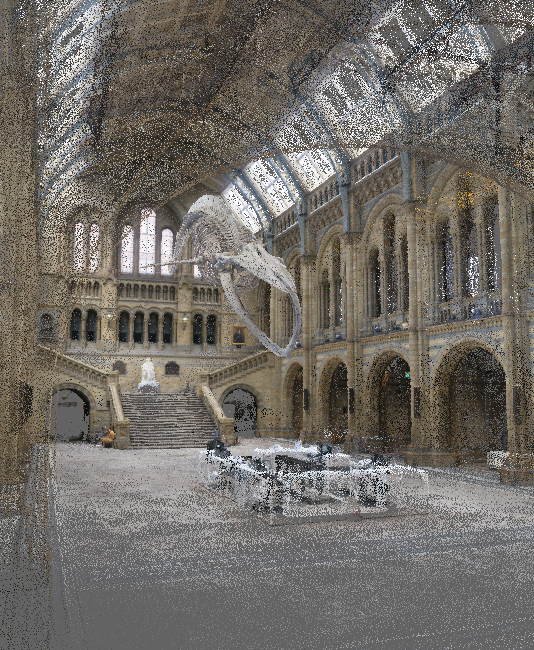
\includegraphics{figs/introduction/hintze.png}
	\caption{Nube de puntos con 2,4M de puntos reconstruidos usando 900 imágenes obtenidas de la Sala Hintze (Modelo subido por \textit{Thomas Flynn} en \textit{Sketchfab}).  }
	\label{fig:hintze_hall_spanish}
\end{marginfigure}
Otro inconveniente de las aplicaciones en tiempo real es la visualización de estos grandes volúmenes de datos. Los métodos tradicionales de rendering están compuesto por un conjunto de etapas inamovibles, en las que la geometría y la topología del modelo se transforman iterativamente para producir una imagen, es decir, píxeles. Los colores de éstos se calculan a partir del sombreado de una o varias fuentes de luz sobre las texturas de una superficie, discretizando la formulación que describe la interacción de la luz. A diferencia de los modelos sintéticos diseñados por operadores humanos, los datos obtenidos por sensores se sombrean en función de la radiancia observada en un conjunto de longitudes de onda a las que es sensible el dispositivo. Por tanto, se necesitan pipelines alternativos para visualizar estos datos. Según la arquitectura de las GPU, los datos pueden ordenarse y organizarse en estructuras de datos buscando un equilibrio entre la carga de trabajo y aquellas simplificaciones geométricas que ayudan a engañar la percepción del usuario. Estos requisitos son aún más exigentes para los dispositivos de Realidad Virtual (RV) que renderizan cada escenario al menos una vez para cada ojo, aunque pueden incrementarse si se incluyen otras técnicas de renderizado, por ejemplo, el mapeado de sombras.   

\marginnote[2cm]{Esta tesis tiene como principal campo de investigación la Agricultura de Precisión y por tanto, el análisis de datos se ha acotado a 1) segmentar los cultivos en suelo y vegetación, y 2) fenotipado de un gran número de variedades vegetales de forma no destructiva.}
Los métodos anteriores no son más que un procedimiento que permite extraer información textual o visual para reconocer puntos débiles y fallos en los procesos. En consecuencia, el último paso es la clasificación, segmentación e identificación de características a partir de los datos de entrada, con el fin optimizar operaciones futuras. Las principales aportaciones de las técnicas de teledetección en la Agricultura de Precisión son la estimación del rendimiento, el inventariado del tipo de cultivo, la medición del contenido de agua, el índice de área foliar (LAI) y el control de enfermedades e insectos, así como la monitorización de la humedad, los cambios, el crecimiento, el estrés y la sequía, entre otros factores de riesgo como la nieve o el fuego \cite{huang_agricultural_2018}. Con estas tareas de vigilancia se pretende maximizar la rentabilidad y minimizar los residuos y la contaminación. 

Se ha publicado un número significativo de conjuntos de datos, junt con la relevancia en auge de la clasificación de imágenes utilizando métodos de aprendizaje automático (ML) y aprendizaje profundo (DL) de inteligencia artificial (IA). Por lo tanto, llevar a cabo tareas de análisis es hoy en día más fácil gracias al acceso a conjuntos de datos de grandes dimensiones. Sin embargo, la mayoría de las grandes colecciones de imágenes de teledetección se basan en sensores espaciales que capturan escenarios muy específicos, por ejemplo, urbanos, en lugar de áreas rurales. Otro reto surge del etiquetado de estas grandes colecciones, dado que debe ser realizado por algoritmos no supervisados, que transforman y extraen características relevantes, o por operadores humanos \cite{li_image_2021, basu_deepsat_2015}. Ninguno de los dos métodos es perfecto y, por tanto, pueden dar lugar a datos incorrectamente clasificados que pueden inducir a error a los algoritmos de aprendizaje. Además, el etiquetado manual se suele realizar sobre bandas visibles, que son más fáciles de interpretar para los humanos, y, por lo tanto, solo unos pocos conjuntos de datos incluyen bandas más allá de R, G, B. En este sentido, los sensores hiperespectrales mitigan este último problema, ya que adquieren conjuntamente un gran número de bandas de las que podemos extraer una imagen en falso color RGB.

Aunque existen algunos conjuntos de datos relevantes para la teledetección, así como una gran variedad de sensores y bandas espectrales, éstos podrían no ser válidos para casos de estudio que no son tan comunes en la literatura. Para solventar esto, se podrían crear conjuntos de datos para aliviar este inconveniente. Sin embargo, adquirir, procesar y extraer características, incluidas las etiquetas, lleva muchísimo tiempo, dado que las tareas manuales requieren recursos informáticos y operadores humanos. Al menos de manera parcial, los datos procedentes de sensores podrían generarse sintéticamente emulando el funcionamiento del sensor. La principal ventaja es que los datos adquiridos a partir de un sensor virtual se vinculan a modelos digitales sin incertidumbre. Asimismo, los modelos digitales se enriquecen con características que podrían transferirse directamente a los resultados de la detección. Los sensores simulados con más frecuencia son los sistemas Radar y LiDAR, aunque recientemente también se han generado imágenes sintéticas con el auge de las redes generativas.

\section{Propósitos y objetivos}

De acuerdo con los retos presentados anteriormente, el objetivo general de esta disertación es contribuir en algunas de las etapas presentadas en la Figura \ref{fig:introduction_scheme_spanish}. Se han revisado brevemente un importante número de retos, entre los que se incluyen un gran número de fuentes de datos heterogéneas, las dificultades en la corrección y fusión de las mismas, la generación de productos con mayor dimensionalidad (por ejemplo, 2D $\rightarrow$ 3D) o el análisis de los resultados finales. De acuerdo con esto, los objetivos de este trabajo son los siguientes:
\begin{itemize}
    \item La corrección y el tratamiento de los datos recogidos mediante misiones de dron. Más que un único frente, este objetivo implica estudiar cómo se pueden corregir todas las fuentes de datos, incluyendo las distorsiones geométricas y radiométricas. La primera debe resolverse en la mayoría de los casos, ya que posibilita la fusión de datos, mientras que la segunda podrá ejecutarse si la radiancia se analiza posteriormente o no.
    \item El emparejamiento de imágenes recogidas por diferentes sensores, dejando atrás las diferencias relativas a 1) la distancia temporal de captura, 2) defectos ópticos, 3) el propio sistema óptico y 4) el intervalo de longitudes de onda adquirido. El emparejamiento de imágenes debe trabajar sobre imágenes con notables cambios de intensidad para obtener matrices de transformación que permitan proyectar una fuente de datos en otra. 
    \item La generación eficiente de grandes nubes de puntos 3D grandes a partir de múltiples fuentes de datos, obteniendo resultados de gran densidad y sin imprecisiones geométricas. La metodología propuesta debería abordar los inconvenientes de los métodos más notables utilizados en la fotogrametría. Además, se trata de una tarea con un alto coste computacional. Esto mismo se ve acentuado por la inclusión de múltiples fuentes de datos, por lo que debe abordarse mediante computación paralela.
    \item A pesar de que los conjuntos de datos anteriores cubren una amplia longitud de onda, éstos se amplían a 3D mediante fotogrametría para obtener un resultado más fácil de comprender. Las técnicas de fotogrametría producen resultados con menor fiabilidad que los productos obtenidos mediante sensores tales LiDAR, el cual recupera directamente la posición tridimensional de la superficie colisionada. La carencia de este sensor entre los disponibles puede resolverse emulándolo sobre escenarios 3D sintéticos. No obstante, esta tarea también requiere mucho tiempo y es especialmente difícil de modelizar en términos de intensidad devuelta. La generación eficiente de grandes conjuntos de datos LiDAR etiquetados debe abordarse, de nuevo, utilizando computación acelerada y caracterizando las superficies modeladas.
    \item La aplicabilidad de las fuentes de datos generadas previamente es el último punto de este trabajo. Entre sus aplicaciones se encuentran la detección de anomalías, la segmentación de materiales o el fenotipado de un gran número de variedades de vegetación. Puede realizarse tanto con técnicas tradicionales, como utilizando modelos de AI
\end{itemize}

\section{Organización del documento}

Esta tesis se compone de seis partes diferentes:

\small \textls[30]{PART I} \normalsize\hspace{3mm} En esta parte se incluye el actual capítulo. Ayuda al usuario a introducirse en la terminología del ámbito de la teledetección, y plantea los principales retos en este campo. A continuación, el Capítulo \ref{sec:fundamentals_rs} ofrece una revisión del estado del arte acerca de la fusión y simulación de datos obtenidos desde un dron.

\small \textls[30]{PART II} \normalsize\hspace{3mm} En esta parte se detallan los conceptos básicos de este trabajo, incluyendo qué tipo de sensores y datos se utilizan. Después, se describe el proceso de corrección y fusión de imágenes que será la base sobre la que se sustenta buena parte de este trabajo (Capítulo \nameref{sec:technology}). En definitiva, esta sección engloba los materiales y métodos que se comparten en múltiple capítulos de este documento.

\small \textls[30]{PART III} \normalsize\hspace{3mm} Esta parte presenta la generación eficiente de nubes de puntos 3D compuestas por múltiples capas: información en el espectro visible, infrarrojo, multiespectral e hiperespectral. La información visible aporta la nube de puntos 3D de referencia, sobre la cual se proyectará el resto de información. En primer lugar, las imágenes infrarrojas se combinan con los datos del espectro visible utilizando computación paralela en la tarjeta gráfica (GPU: Graphics Processing Unit). Un procedimiento muy similar se muestra consecutivamente para proyectar la información multiespectral, aunque esta última presenta algunos desafíos adicionales procedentes de la alineación de múltiples imágenes en intervalos espectrales muy distintos. Por último, la nube de puntos hiperespectral se genera siguiendo una metodología adaptada a unas condiciones de adquisición de datos hiperespectrales muy específicas.

\small \textls[30]{PART IV} \normalsize\hspace{3mm} Una vez se han obtenido los resultados utilizando aquellos sensores disponibles, se plantea la simulación de aquellos otros sensores cuyo acceso es prohibitivo, y de los cuáles aún no disponía el grupo de investigación. Más en concreto, nos centramos en la simulación de LiDAR, utilizando escenarios sintéticos con etiquetas semánticas. La simulación LiDAR se describe en dos capítulos, centrados en 1) la simulación de las propiedades geométricas de una nube de puntos LiDAR (Capítulo \ref{sec:lidar_simulation}) y 2) la simulación de la radiancia observada en el Capítulo \ref{sec:lidar_intensity}). Después, la simulación se emplea en la optimización de escaneos terrestres, principalmente en edificios, indicando qué posiciones son las óptimas de acuerdo a la configuración del sensor. Este proceso de optimización se describe en el Capítulo \ref{sec:lidar_optimization}, y aunque se aplica a edificios, no plantea ninguna restricción para poder aplicarlo a cualquier otro tipo de entorno.

\small \textls[30]{PART V} \normalsize\hspace{3mm} Esta parte muestra algunas aplicaciones de las nubes de puntos térmicas y las imágenes hiperespectrales. Las primeras se aplican a la detección de anomalías térmicas, relacionados con restos arqueológicos que pudieran haber pasado desapercibidos. Por otro lado, la información hiperespectral se corrige y procesa para ser aplicada a la identificación automática de variedades de viñedos, utilizando modelos de Inteligencia Artificial. 

\small \textls[30]{PART VI} \normalsize\hspace{3mm} El Capítulo \ref{sec:conclusions} concluye este trabajo mostrando los principales resultados obtenidos, así como las posibles líneas futuras de trabajo.